\documentclass{article}
\usepackage{makeidx}
\usepackage{hyperref}
\usepackage{amsmath}
\usepackage{amssymb}
\usepackage{xcolor}
\usepackage{graphicx}

\title{Deep Learning Notes}
\author{Haotian Chen}
\date{}

\makeatletter
\renewcommand\paragraph{\@startsection{paragraph}{4}{\z@}%
                                     {-3.25ex\@plus -1ex \@minus -.2ex}%
                                     {1.5ex \@plus .2ex}%
                                     {\normalfont\normalsize\bfseries}}
\makeatletter

\hypersetup{
    colorlinks=true,
    linkcolor=blue,
    urlcolor=cyan,
}

\setcounter{tocdepth}{4}
\setcounter{secnumdepth}{4}

\makeindex



\begin{document}

\maketitle

\clearpage

\tableofcontents{}

\clearpage

\section{Neural Networks and Deep Learning}

\subsection{Activation Function}

\noindent \textbf{binary step:}

\begin{center}
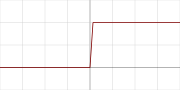
\includegraphics[scale=0.8]{./images/binary_step.png}
\end{center}

\[f(x) = \begin{cases}0&{\text{if }}x<0\\1&{\text{if }}x\geq 0\end{cases}, f(x) \in \{0, 1\}\]
\[f'(x) = \begin{cases}0&{\text{if }}x\neq 0\\{\text{undefined}}&{\text{if }}x=0\end{cases}\]

\noindent \textbf{sigmoid function:} (mainly used in output layer)

\begin{center}
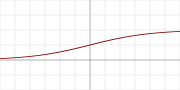
\includegraphics[scale=0.8]{./images/sigmoid.png}
\end{center}

\[f(x) = \sigma (x)={\frac {e^{x}}{e^{x}+1}}={\frac {1}{1+e^{-x}}}, f(x) \in (0, 1)\]
\[f'(x) = f(x)(1-f(x))\]

\noindent \textbf{rectified linear unit:}  (relu, mainly used in hidden layer)

\begin{center}
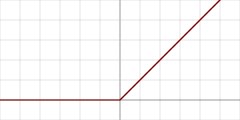
\includegraphics[scale=0.6]{./images/relu.png}
\end{center}

\[f(x) = max\{0, x\} = \begin{cases}0&{\text{if }}x<0\\1&{\text{if }}x\geq 0\end{cases}, f(x) \in [0, +\infty)\]
\[f'(x) = \begin{cases}0&{\text{if }}x<0\\1&{\text{if }}x>0\\{\text{undefined}}&{\text{if }}x=0\end{cases}\]

\noindent \textbf{Leaky rectified linear unit:}  (leaky relu, mainly used in hidden layer)

\begin{center}
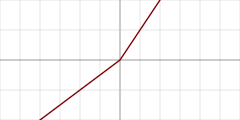
\includegraphics[scale=0.6]{./images/leaky_relu.png}
\end{center}

\[f(x) = \begin{cases}0.01x&{\text{if }}x<0\\x&{\text{if }}x\geq 0\end{cases}, f(x) \in (- \infty, + \infty)\]
\[f'(x) = \begin{cases}0.01&{\text{if }}x<0\\1&{\text{if }}x\geq 0\end{cases}\]

\noindent \textbf{hyperbolic tangent:} (tanh, mainly used in hidden layer)

\begin{center}
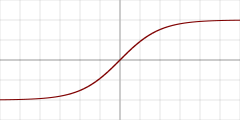
\includegraphics[scale=0.6]{./images/tanh.png}
\end{center}

\[f(x) = \tanh(x) = \frac {e^{x}-e^{-x}}{e^{x}+e^{-x}}, f(x) \in (-1, 1)\]
\[f'(x) = 1-f(x)^{2}\]

\noindent It turns out that the tanh activation usually works better than sigmoid activation function for hidden units because the mean of its output is closer to zero, and so it centers the data better for the next layer. Sigmoid or Tanh function disadvantage is that if the input is too small or too high, the slope will be near zero which will cause us the vanishing gradient problem.

\bigskip

\noindent Linear activation function will output linear activations. No matter how many hidden layers you add, the activation will be always linear like logistic regression (So its useless in a lot of complex problems). You might use linear activation function in the output layer if the output is real numbers (regression problem).

\subsection{Computation Graphs of Derivatives:}

\begin{center}
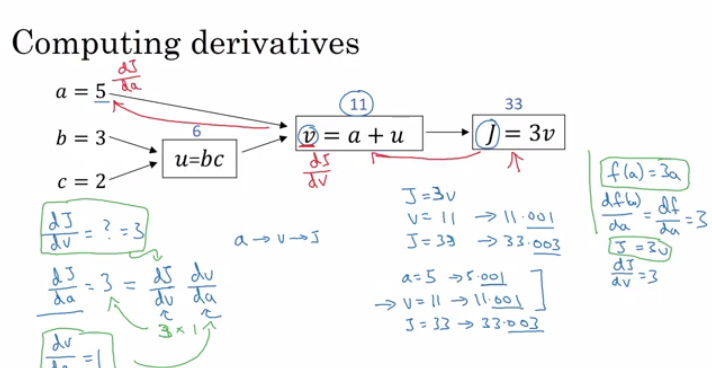
\includegraphics[scale=0.6]{./images/computation_graph.png}
\end{center}

\noindent apply chain rule:

\[\frac{\partial J}{\partial a} = \frac{\partial J}{\partial v} \frac{\partial v}{\partial a} = 3 \times 1 = 3\]

\[\frac{\partial J}{\partial b} = \frac{\partial J}{\partial v} \frac{\partial v}{\partial u} \frac{\partial u}{\partial b} = 3 \times 1 \times 2 = 6\]

\[\frac{\partial J}{\partial c} = \frac{\partial J}{\partial v} \frac{\partial v}{\partial u} \frac{\partial u}{\partial c} = 3 \times 1 \times 3 = 9\]


\subsection{Binary Classification}

Use logistic regression to build a binary classifier.

\begin{center}
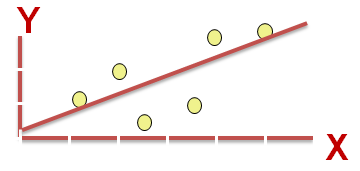
\includegraphics[scale=0.4]{./images/binary_classification.png}
\end{center}

\noindent \textbf{training data:}
\[x \in \mathbb{R}^{n_x}, y \in \{0, 1\}\]
\[\text{\(m\) training examples: } (x^{(i)}, y^{(i)})\:for\:i = 1, \dots, m\]

\[
x^{(i)} = 
\begin{bmatrix}
x^{(i)}_1\\
x^{(i)}_2\\
\vdots\\
x^{(i)}_n
\end{bmatrix}
,
y^{(i)} = y^{(i)}_1
\]

\[X =
\begin{bmatrix}
x^{(1)} & x^{(2)} & \dots & x^{(m)}
\end{bmatrix}
,
Y =
\begin{bmatrix}
y^{(1)} & y^{(2)} & \dots & y^{(m)}
\end{bmatrix}
\]

\[X \in \mathbb{R}^{n_x \times m}, Y \in \mathbb{R}^{1 \times m}\]

\subsection{Logistic Regression}

\noindent Logistic regression is a statistical model that uses a logistic function to model a binary dependent variable.

\bigskip

\noindent Given \(x\), want \(\hat{y} = P(y = 1 | x)\), where \(0 \leq \hat{y} \leq 1\), \(x \in \mathbb{R}^{n_x}\), \(w \in \mathbb{R}^{n_x}\), \(b \in \mathbb{R}\)

\[z = w^Tx + b\]
\[\hat{y} = \sigma(z) = \frac {1}{1+e^{-z}}\]

\[P(y|x) = \begin{cases}\hat{y}&{\text{if }}y = 1\\1 -\hat{y}&{\text{if }}y = 0\end{cases} = \hat{y}^y (1 - \hat{y})^{(1 - y)}\]

\noindent We want to maximize \(P(y|x)\). To make it simpler, because \(log\) function is a strictly increasing function, we can maximize \(log(P(y|x))\) instead.

\[log(P(y|x)) = log(\hat{y}^y (1 - \hat{y})^{(1 - y)}) = ylog(\hat{y}) + (1 - y)log(1 - \hat{y})\]

\noindent Or in reverse, we can minimize \(-log(P(y|x))\), which is called \textbf{loss function}.

\noindent \textbf{loss function: (convex)}

\[L(\hat{y}, y) = -(ylog(\hat{y}) + (1 - y)log(1 - \hat{y}))\]

\noindent \textbf{cost function: (convex)}

\[J(w, b) = \frac{1}{m} \sum^m_{i = 1} L(\hat{y}^{(i)}, y^{(i)}) = - \frac{1}{m} \sum^m_{i = 1} [y^{(i)}log(\hat{y}^{(i)}) + (1 - y^{(i)})log(1 - \hat{y}^{(i)})]\]

\noindent \textbf{gradient descent:} with learning rate \(\alpha\), find best \(w\), \(b\) to minimize \(J(w, b)\)

\noindent repeat until convergence \{
\[w_j =: w_j - \alpha \frac{\partial}{\partial w_j} J(w, b) = w_j - \alpha \frac{1}{m} \sum^m_{i = 1} (\hat{y}^{(i)} - y^{(i)}) x^{(i)}_j\]
\[b =: b - \alpha \frac{\partial}{\partial b} J(w, b) = b - \alpha \frac{1}{m} \sum^m_{i = 1} (\hat{y}^{(i)} - y^{(i)})\]
\centerline{simultaneously update \(w_j\) and \(b\), \(j \in [1, n]\)}
\}

\bigskip

\noindent \textbf{vectorized implementation}:

\noindent repeat until convergence \{
\[w =: w - \alpha \frac{1}{m} X (\sigma(w^TX + b) - Y)^T\]
\[b =: b - \alpha \frac{1}{m} sum\{\sigma(w^TX + b) - Y\}\]
\}

\subsection{Neural Network}

\noindent \textbf{Basic Structure:}

\begin{center}
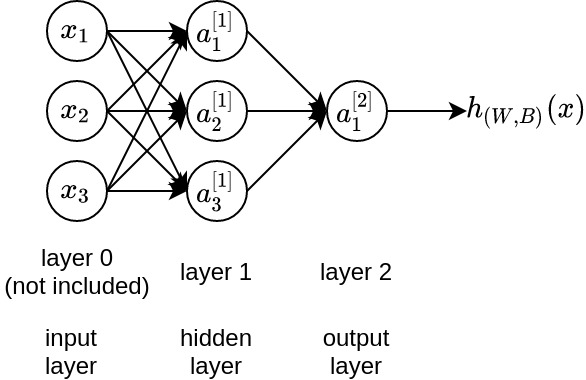
\includegraphics[scale=0.4]{./images/neural_network.jpg}
\end{center}
\[a_i^{[j]} = \text{"activation" of unit i in layer j}\]
\[W^{[j]} = \text{matrix of weights (edges) from layer j - 1 to j}\]
\[B^{[j]} = \text{vector of biases (nodes) from layer j - 1 to j}\]

\[a_1^{[1]} = \sigma(W_{11}^{[1]} x_1 + W_{12}^{[1]} x_2 + W_{13}^{[1]} x_3 + B_{1}^{[1]})\]
\[a_2^{[1]} = \sigma(W_{21}^{[1]} x_1 + W_{22}^{[1]} x_2 + W_{23}^{[1]} x_3 + B_{2}^{[1]})\]
\[a_3^{[1]} = \sigma(W_{31}^{[1]} x_1 + W_{32}^{[1]} x_2 + W_{33}^{[1]} x_3 + B_{3}^{[1]})\]
\[h_{(W, B)}(x) = a_1^{[2]} = \sigma(W_{11}^{[2]} a_1^{[1]} + W_{12}^{[2]} a_2^{[1]} + W_{13}^{[2]} a_3^{[1]} + B_{1}^{[2]})\]

\bigskip

\noindent If network has \(s_j\) units in layer \(j\), \(s_{j - 1}\) units in layer \(j - 1\), then \(W^{[j]}\) will be of dimension \(s_j \times s_{j - 1}\), \(B^{[j]}\) will be of dimension \(s_j \times 1\).

\bigskip

\noindent \textbf{Generalized Model (one vs all):}

\begin{center}
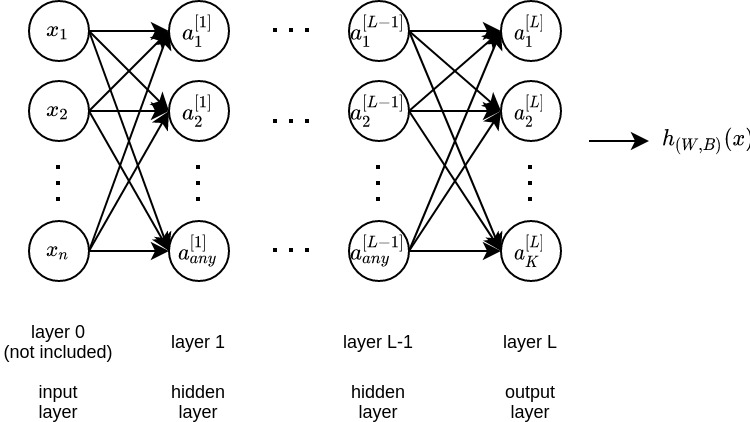
\includegraphics[scale=0.4]{./images/neural_network_generalized.jpg}
\end{center}

\noindent For a neural network that has:

\[L = \text{total number of layers in the network}\]
\[s_l = \text{number of units in layer } l\]
\[K = \text{number of output units/classes}\]

\noindent assume \(a^{[0]} = x, a^{[L]} = h_{(W, B)}(x)\), let:

\[z^{[l]} = W^{[l]} a^{[l - 1]} + B^{[l]}\]
\[a^{[l]} = \sigma(z^{[l]})\]
\[h_{(W, B)}(x) = a^{[L]} = \sigma(z^{[L]})\]

\bigskip

\noindent \textbf{regularized cost function:}
\[J(W, B) = - \frac{1}{m} \sum_{i = 1}^{m} \sum_{k = 1}^{K} [y^{(i)}_k log(h_{(W, B)} (x^{(i)})_k) + (1 - y^{(i)}_k) log(1 - h_{(W, B)}(x^{(i)})_k)] + \frac{\lambda}{2m} \sum_{l = 1}^{L} \sum_{i = 1}^{s_l} \sum_{j = 1}^{s_{l + 1}} (W_{j, i}^{[l]})^{2}\]

\noindent To reduce over-fitting, we can reduce(penalize) the weight of the features in our function carry by increasing their cost. The \(\lambda\) is the regularization parameter. It determines how much the costs of our theta parameters are inflated.

\bigskip

\noindent \textbf{vectorized implementation}: (with different activation function for each layer)

\[Z^{[l]} = W^{[l]}A^{[l - 1]} + B^{[l]}\]
\[A^{[l]} = \sigma^{[l]}(Z^{[l]})\]
\[h_{(W, B)}(X) = A^{[L]} = \sigma^{[L]}(Z^{[L]})\]
\[J(W, B) =  - \frac{1}{m} np.sum(Y \odot log(h_{(W, B)}(X)) + (1 - Y) \odot log(1 - h_{(W, B)}(X))) + \frac{\lambda}{2m} np.sum(W \odot W)\]

\subsection{Backpropagation Preliminary}
\noindent \textbf{matrix calculus:} see \href{https://en.wikipedia.org/wiki/Matrix_calculus}{Wikipedia}

\noindent \textbf{chaine rule:}

\noindent Suppose the variable \(J\) depends on the variables \(w_1, \dots, w_p\) via the intermediate variable \(z_1, \dots, z_k\).

\[z_j = z_j(w_1, \dots, w_p), \forall j \in \{1, \dots, k\} \]
\[J = J(z_1, \dots, z_k)\]

\noindent Expand \(J\), we can find:

\[\frac{\partial J}{\partial w_i} = \sum_{j = 1}^{k} \frac{\partial J}{\partial z_j} \frac{\partial z_j}{\partial w_i}, \forall i \in \{1, \dots, p\}\]

\noindent \textbf{chain rule derivation for matrix:}

\noindent Suppose \(J\) is a real-valued output variable, \(z \in \mathbb{R}^m\) is the intermediate variable and \(W \in \mathbb{R}^{m \times d}\), \(B \in \mathbb{R}^{m}\), \(a \in \mathbb{R}^d\) are the input variables. Suppose they satisfy:

\[z = W a + B\]
\[J = J(z)\]

\noindent Then we can get:

\[
\frac{\partial J}{\partial a} = 
\begin{bmatrix}
\frac{\partial J}{\partial a_1}\\
\vdots\\
\frac{\partial J}{\partial a_d}
\end{bmatrix}
= 
\begin{bmatrix}
\sum_{j = 1}^m \frac{\partial J}{\partial z_j} \frac{z_j}{a_1}\\
\vdots\\
\sum_{j = 1}^m \frac{\partial J}{\partial z_j} \frac{z_j}{a_d}
\end{bmatrix}
=
\begin{bmatrix}
\frac{\partial z_1}{\partial a_1} & \dots & \frac{\partial z_m}{\partial a_1}\\
\vdots & \ddots & \vdots\\
\frac{\partial z_1}{\partial a_d} & \dots & \frac{\partial z_m}{\partial a_d}
\end{bmatrix}
\begin{bmatrix}
\frac{\partial J}{\partial z_1}\\
\vdots\\
\frac{\partial J}{\partial z_m}
\end{bmatrix}
= \frac{\partial z}{\partial a} \frac{\partial J}{\partial z}
= W^T \frac{\partial J}{\partial z}
\]

\[
\frac{\partial J}{\partial W_{ij}} = \sum_{k = 1}^m \frac{\partial J}{\partial z_k} \frac{\partial z_k}{\partial W_{ij}} = \frac{\partial J}{\partial z_i} \frac{\partial z_i}{\partial W_{ij}} = \frac{\partial J}{\partial z_i} a_j
\]

\[
\frac{\partial J}{\partial B_{i}} = \sum_{k = 1}^m \frac{\partial J}{\partial z_k} \frac{\partial z_k}{\partial B_{i}} = \frac{\partial J}{\partial z_i} \frac{\partial z_i}{\partial B_{i}} = \frac{\partial J}{\partial z_i}
\]

\[
\frac{\partial J}{\partial W} = 
\begin{bmatrix}
\frac{\partial J}{\partial z_1}\\
\vdots\\
\frac{\partial J}{\partial z_m}
\end{bmatrix}
\begin{bmatrix}
a_1 & \dots & a_d
\end{bmatrix}
= \frac{\partial J}{\partial z} a^T
\]

\[
\frac{\partial J}{\partial B} = 
\begin{bmatrix}
\frac{\partial J}{\partial z_1}\\
\vdots\\
\frac{\partial J}{\partial z_m}
\end{bmatrix}
= \frac{\partial J}{\partial z}
\]

\noindent \textbf{element-wise chain rule:}

\noindent Assume \(z, a \in \mathbb{R}^d\):

\[a = \sigma(z) \text{, where \(\sigma\) is an element-wise activation}\]
\[J = J(a)\]

\noindent Then we have:

\[\frac{\partial J}{\partial z} = \frac{\partial J}{\partial a} \odot \sigma'(z)\]

\noindent Where \(\sigma'\) is the element-wise derivative of the activation function \(\sigma\).

\subsection{Backpropagation}

\noindent To train the model, we need to update \(W\) and \(B\) for each epoch: (gradient decent)

\[W := W - \alpha  \frac{\partial}{\partial W} J(W, B)\]
\[B := B - \alpha  \frac{\partial}{\partial B} J(W, B)\]

\noindent We can see \(\frac{\partial}{\partial W} J(W, B)\) and \(\frac{\partial}{\partial B} J(W, B)\) are hard to get directly. There is an easier way to calculate it. For each training example \((x^{(q)}, y^{(q)}), q \in \{1, \dots, m\}\), define \textbf{loss function}:

\[J = -\sum_{k = 1}^{K} [y^{(q)}_k log(h_{(W, B)} (x^{(q)})_k) + (1 - y^{(q)}_k) log(1 - h_{(W, B)}(x^{(q)})_k)] \]

\noindent Apply chain rule we have:

\[\frac{\partial J}{\partial W^{[l]}} = \frac{\partial J}{\partial z^{[l]}} (a^{[l - 1]})^T\]
\[\frac{\partial J}{\partial B^{[l]}} = \frac{\partial J}{\partial z^{[l]}}\]
\[\frac{\partial J}{\partial a^{[l]}} = (W^{[l + 1]})^T \frac{\partial J}{\partial z^{[l + 1]}}\]
\begin{equation*}
\begin{split}
\frac{\partial J}{\partial z^{[l]}}
& = \frac{\partial J}{\partial a^{[l]}} \odot \sigma'(z^{[l]}) \\
& = (W^{[l + 1]})^T \frac{\partial J}{\partial z^{[l + 1]}} \odot \sigma'(z^{[l]}) \\
& = (W^{[l + 1]})^T \frac{\partial J}{\partial z^{[l + 1]}} \odot (a^{[l]} \odot (1 - a^{[l]}))
\end{split}
\end{equation*}

\noindent For \(p \in \{1, ..., K\}\):
\begin{equation*}
\begin{split}
\frac{\partial J}{\partial z_p^{[L]}} 
& = \frac{\partial}{\partial z_p^{[L]}} \sum_{k = 1}^{K} -[y^{(q)}_k log(h_{(W, B)} (x^{(q)})_k) + (1 - y^{(q)}_k) log(1 - h_{(W, B)}(x^{(q)})_k)] \\
& = \frac{\partial}{\partial z_p^{[L]}} \{-[y^{(q)}_p log(\frac{1}{1 + e^{-z_p^{[L]}}}) + (1 - y^{(q)}_p) log(1 - \frac{1}{1 + e^{-z_p^{[L]}}})]\} \\
& = - [y^{(q)}_p (1 + e^{-z_p^{[L]}}) \frac{0 - (-e^{-z_p^{[L]}})}{(1 + e^{-z_p^{[L]}})^2} + (1 - y^{(q)}_p) \frac{1 + e^{-z_p^{[L]}}}{e^{-z_p^{[L]}}} \frac{(-e^{-z_p^{[L]}})(1 + e^{-z_p^{[L]}}) - e^{-z_p^{[L]}}(-e^{-z_p^{[L]}})}{(1 + e^{-z_p^{[L]}})^2}] \\
& = - [y_p^{(q)} \frac{e^{-z_p^{[L]}}}{1 + e^{-z_p^{[L]}}} + (1 - y_p^{(q)}) \frac{-1}{1 + e^{-z_p^{[L]}}}] \\
& = - \frac{y_p^{(q)}e^{-z_p^{[L]}} + y_p^{(q)} - 1}{1 + e^{-z_p^{[L]}}} \\
& = \frac{1}{1 + e^{-z_p^{[L]}}} - y_p^{(q)} \\ 
& = a_p^{[L]} - y_p^{(q)}
\end{split}
\end{equation*}

\noindent Then we get:

\[\frac{\partial J}{\partial z^{[L]}} = 
\begin{bmatrix}
\frac{\partial J}{\partial z_1^{[L]}} \\
\vdots \\
\frac{\partial J}{\partial z_K^{[L]}}
\end{bmatrix}
= a^{[L]} - y^{(q)}
\]

\noindent For convenience, define \textbf{error term}: 
\[\delta^{[l]} = \frac{\partial J}{\partial z^{[l]}}\]

\noindent Then we get:

\[\frac{\partial J}{\partial W^{[l]}} = \delta^{[l]} (a^{[l - 1]})^T\]
\[\frac{\partial J}{\partial B^{[l]}} = \delta^{[l]}\]
\[\delta^{[l]} = (W^{[l + 1]})^T \delta^{[l + 1]} \odot (a^{[l]} \odot (1 - a^{[l]}))\]
\[\delta^{[L]} = a^{[L]} - y^{(q)}\]

\noindent \textbf{backpropagation algorithm:} (compute \(\frac{\partial}{\partial W} J(W, B)\), \(\frac{\partial}{\partial B} J(W, B)\))

\noindent training set: \((x^{(q)}, y^{(q)}), q \in \{1, \dots, m\}\)

\noindent set \(\Delta(W)_{ij}^{[l]} = 0, \Delta(B)_{i}^{[l]} = 0, l \in \{1, \dots, L\}\)

\noindent for \(q \in \{1, \dots, m\}\):

\noindent \hspace{.5cm} forward propagation: compute \(a^{[l]}\) for \(l \in \{1, \dots, L\}\)

\noindent \hspace{.5cm} compute \(\delta^{[L]} = \frac{\partial J}{\partial z^{[L]}} = a^{[L]} - y^{(q)}\)

\noindent \hspace{.5cm} for \(l \in \{L - 1, \dots, 1\}\):

\noindent \hspace{1cm} compute \(\delta^{[l]} = (W^{[l + 1]})^T \delta^{[l + 1]} \odot \sigma'(z^{[l]}) = (W^{[l + 1]})^T \delta^{[l + 1]} \odot (a^{[l]} \odot (1 - a^{[l]}))\)

\noindent \hspace{.5cm} for \(l \in \{1, \dots, L\}\):

\noindent \hspace{1cm} compute \(\Delta(W)^{[l]} := \Delta(W)^{[l]} + \frac{\partial J}{\partial W^{[l]}} = \Delta(W)^{[l]} + \delta^{[l]}(a^{[l - 1]})^T\)

\noindent \hspace{1cm} compute \(\Delta(B)^{[l]} := \Delta(B)^{[l]} + \frac{\partial J}{\partial B^{[l]}} = \Delta(B)^{[l]} + \delta^{[l]}\)

\noindent compute \(\frac{\partial}{\partial W_{ij}^{[l]}} J(W, B) = D(W)_{ij}^{[l]} = \frac{1}{m} \Delta(W)_{ij}^{[l]} + \frac{\lambda}{m} W_{ij}^{[l]}\)

\noindent compute \(\frac{\partial}{\partial B_{i}^{[l]}} J(W, B) = D(B)_{i}^{[l]} = \frac{1}{m} \Delta(B)_{i}^{[l]}\)

\bigskip

\noindent \textbf{vectorized backpropagation algorithm:} (compute \(\frac{\partial}{\partial W} J(W, B)\), \(\frac{\partial}{\partial B} J(W, B)\))

\noindent with different activation function for each layer:

\[\partial Z^{[L]} = \frac{\partial}{\partial Z^{[L]}} J(W, B) = A^{[L]} - Y\]
\[\partial Z^{[l]} = \frac{\partial}{\partial Z^{[l]}} J(W, B) = (W^{[l + 1]})^T \partial Z^{[l + 1]} \odot \sigma'^{[l]}(Z^{[l]})\]
\[\partial W^{[l]} = \frac{\partial}{\partial W^{[l]}} J(W, B) = \frac{1}{m} \partial Z^{[l]} (A^{[l - 1]})^T + \frac{\lambda}{m} W^{[l]}\]
\[\partial B^{[l]} = \frac{\partial}{\partial B^{[l]}} J(W, B) = \frac{1}{m} np.sum(\partial Z^{[l]}, axis=1, keepdims=True)\]

\subsection{Random Initialization (symmetry breaking)}

\noindent Initializing bias matrices \(B\) with zero is OK. Initializing all the weight matrices \(W\) with zero does not work with neural networks, because all hidden units will be completely identical (symmetric) - compute exactly the same function. When we backpropagate, all nodes will update to the same value repeatedly. Instead we can randomly initialize our weights for our \(W\) matrices using the following method: (here \(\epsilon\) is a value selected for random initialization)

\[\text{initialize each } W_{ij}^{[l]} \text{ to a random value in } [-\epsilon, +\epsilon]\]

\noindent One effective strategy for choosing \(\epsilon\) is to base it on the number of units in the network: (Xavier normalized initialization)

\[\epsilon^{[l]} = \frac{\sqrt{6}}{\sqrt{s^{[l]} + s^{[l - 1]}}}\]

\subsection{Parameters vs Hyperparameters}

\noindent Main parameters of the Neural Network are \(W\) and \(B\).

\noindent Hyper parameters (parameters that used to find best main parameters) are like:

\begin{itemize}
  \item Learning rate.
  \item Number of iteration.
  \item Number of hidden layers.
  \item Number of hidden units.
  \item Choice of activation functions.
  \item Momentum term.
  \item Mini-batch size.
  \item Regularization parameters.
\end{itemize}

\section{Hyperparameter Tuning, Regularization and Optimization}

\subsection{Train/Dev/Test Sets}

\noindent \textbf{find better hyperparameters}:

\noindent repeat: Idea \(\longrightarrow\) Code \(\longrightarrow\) Experiment

\bigskip

\noindent \textbf{split dataset}:

\begin{itemize}
  \item Training set
  \item Validation set / Development or "dev" set.
  \item Testing set
\end{itemize}

\noindent \textbf{ratio of splitting}:
\begin{itemize}
  \item If size of the dataset is 100 to 1000000: 60\%/20\%/20\%
  \item If size of the dataset is 1000000 to INF: 98\%/1\%/1\% or 99.5\%/0.25\%/0.25\%
\end{itemize}

\noindent Make sure the dev and test set are coming from the same distribution. For example if cat training pictures is from the web and the dev/test pictures are from users cell phone they will mismatch. It is better to make sure that dev and test set are from the same distribution.

\bigskip

\noindent The dev set rule is to try them on some of the good models you've created. Its OK to only have a dev set without a testing set. But a lot of people in this case call the dev set as the test set. A better terminology is to call it a dev set as its used in the development.

\subsection{Bias/Variance}

\noindent The training error will tend to decrease as we increase the degree \(d\) of the polynomial. At the same time, the cross validation error will tend to decrease as we increase \(d\) up to a point, and then it will increase as \(d\) is increased, forming a convex curve.

\begin{center}
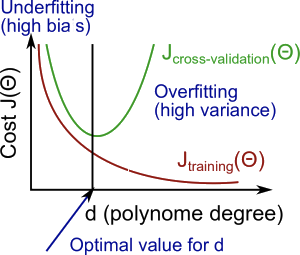
\includegraphics[scale=0.4]{./images/bias_and_variance_polynomial.png}
\end{center}

\noindent High bias(underfitting): both \(J_{train}(W, B)\) and \(J_{cv}(W, B)\) will be high. Also, \(J_{cv}(W, B) \approx J_{train}(W, B)\). 

\noindent High variance(overfitting): \(J_{train}(W, B)\) will be low and \(J_{cv}(W, B)\) will be high. Also, \(J_{cv}(W, B) \gg J_{train}(W, B)\). 

\bigskip

\noindent \textbf{underfitting}:

\noindent High bias, which means hypothesis fits training data poorly, is usually caused by a function that is too simple or using too few features. 

\bigskip

\noindent \textbf{overfitting}:

\noindent High variance, which means hypothesis fits training data well, but does not generalize well to predict new data. It is usually caused by a complicated function with too many features.

\subsection{Basic Recipe for Machine Learning}

\noindent If your algorithm has a high bias:

\begin{itemize}
  \item Try to make your NN bigger (size of hidden units, number of layers)
  \item Try a different model that is suitable for your data.
  \item Try to run it longer.
  \item Different (advanced) optimization algorithms.
\end{itemize}

\noindent If your algorithm has a high variance:

\begin{itemize}
  \item More data.
  \item Try regularization.
  \item Try a different model that is suitable for your data.
\end{itemize}

\noindent You should try the previous two points until you have a low bias and low variance. In the older days before deep learning, there was a "Bias/variance tradeoff". But because now you have more options/tools for solving the bias and variance problem its really helpful to use deep learning. With enough training data, training a bigger neural network never hurts.

\bigskip

\noindent \textbf{Regularization}: (L2 Regularization) 

\noindent Add regularization term to the cost function to reduce variance (overfitting):

\[\frac{\lambda}{2m} \sum_{l = 1}^{L} \sum_{i = 1}^{s_l} \sum_{j = 1}^{s_{l + 1}} (W_{j, i}^{[l]})^{2} = \frac{\lambda}{2m} np.sum(W \odot W)\]

\bigskip

\noindent weight backpropagation with regularization:

\[W^{[l]} := W^{[l]} - \alpha \partial W^{[l]} = (1 - \frac{\alpha \lambda}{m}) W^{[l]} - \frac{\alpha}{m} \partial Z^{[l]} (A^{[l - 1]})^T\]

\noindent The new term \((1 - \frac{\alpha \lambda}{m}) W^{[l]}\) causes the weight to decay in proportion to its size. In practice this penalizes large weights and effectively limits the freedom in your model.


\begin{itemize}
  \item If \(\lambda\) is too large - \(W^{[l]}_{i,j}\) will be close to zeros which will make the NN simpler.
  \item If \(\lambda\) is good enough it will just reduce some weights and prevent the overfitting.
  \item If \(\lambda\) is too large, \(Z^{[l]}_{i}\) will be small (close to zero) - assume tanh activation function is used, then it will behave like a linear function, so we will go from non linear activation to roughly linear which would make the NN a roughly linear classifier.
  \item If \(\lambda\) good enough it will just make some of tanh activations roughly linear which will prevent overfitting.
\end{itemize}

\noindent Implementation tip: if you implement gradient descent, plot the cost function as a function of the number of iterations of gradient descent and you want to see that the cost function decreases monotonically after every elevation of gradient descent with regularization.

\bigskip

\noindent \textbf{Dropout}:

\noindent The dropout regularization eliminates some neurons/weights on each iteration based on a probability. It is used to reduce overfitting. A most common technique to implement dropout is called "Inverted dropout".

\[keep\_prob = 0.8 \text{ (for example)}\]
\[D^{[l]} = np.random.rand(A^{[l]}.shape[0], A^{[l]}.shape[1]) < keep\_prob\]
\[A^{[l]} = A^{[l]} \odot D^{[l]}\]
\[A^{[l]} = keep\_prob^{-1} A^{[l]}\]

\begin{center}
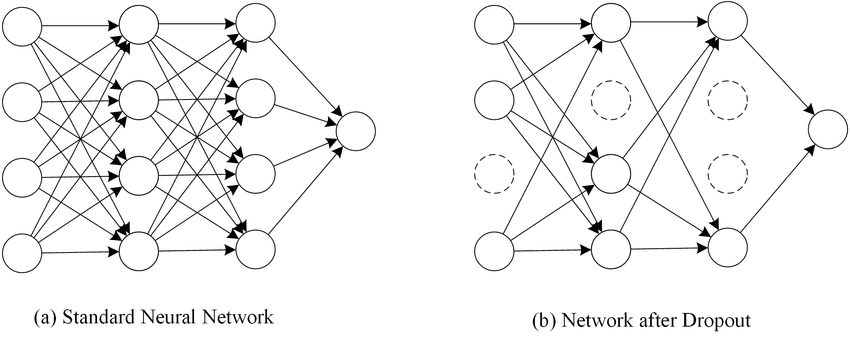
\includegraphics[scale=0.4]{./images/dropout_neural_network.png}
\end{center}

\noindent Drop 20\% of units in \(A^{[l]}\) by replacing them with 0, then scale \(A^{[l]}\) by \(keep\_prob^{-1}\). 

\bigskip

\noindent We need to scale \(A^{[l]}\) because \(Z^{[l + 1]} = W^{[l + 1]} A^{[l]} + B^{[l + 1]}\). And we want to increase \(A^{[l]}\) to not reduce the expected value of output \(Z^{[l + 1]}\) after dropout.

\bigskip

\noindent \(D^{[l]}\) is used for forward and back propagation and is the same for them, but it is different for each iteration of training example. At test time we don't use dropout. Otherwise it would add noise to predictions.

\bigskip

\noindent \textbf{Understanding Dropout}:

\begin{itemize}
  \item The intuition is dropout randomly knocks out units in your network. So it's as if on every iteration you're working with a smaller NN, and so using a smaller NN seems like it should have a regularizing effect.
  \item Another intuition: can't rely on any single feature, so have to spread out weights.
  \item Dropout can have different keep\_prob per layer.
  \item The input layer dropout has to be near 1 (or 1 - no dropout) because you don't want to eliminate a lot of features.
  \item If you're more worried about some layers overfitting than others, you can set a lower keep\_prob for some layers than others. The downside is, this gives you even more hyperparameters to search for using cross-validation. One other alternative might be to have some layers where you apply dropout and some layers where you don't apply dropout and then just have one hyperparameter, which is a keep\_prob for the layers for which you do apply dropouts.
  \item A lot of researchers are using dropout with Computer Vision (CV) because they have a very big input size and almost never have enough data, so overfitting is the usual problem.
  \item A downside of dropout is that the cost function is not well defined and it will be hard to debug (plot cost by iteration). To solve that you'll need to turn off dropout, set all the keep\_prob to 1, and then run the code and check that it monotonically decreases cost and then turn on the dropouts again.
\end{itemize}

\noindent \textbf{Other regularization methods}:

\begin{itemize}
  \item Data augmentation. For example, you can flip all your pictures horizontally this will give you m more data instances. You could also apply a random position and rotation to an image to get more data. New data obtained using this technique isn't as good as the real independent data, but still can be used as a regularization technique.
  \item Early stopping. We will pick the point at which the training set error and dev set error are best (lowest training cost with lowest dev cost). We will take these parameters as the best parameters.
\end{itemize}

\noindent \textbf{Normalizing Inputs}: (Feature Scaling)

\noindent All features should be normalized so that they are scaled into a certain range and each feature contributes approximately proportionately to the result. It helps to center the dataset. Also it helps gradient descent converge much faster.

\bigskip

\noindent This should be applied to training, dev, and testing sets (but using mean and variance of the training set).

\begin{center}
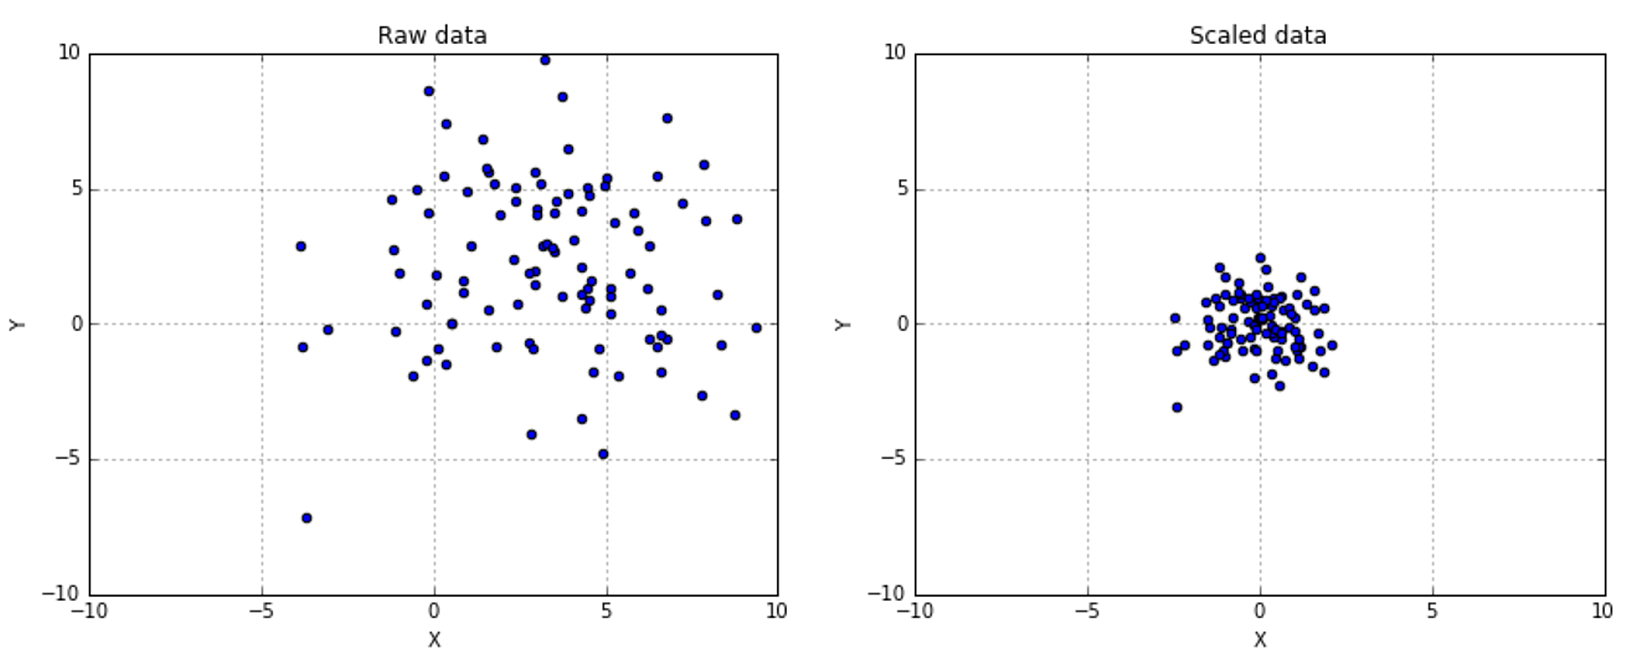
\includegraphics[scale=0.8]{./images/normalize_input.png}
\end{center}

\noindent If we normalize inputs, the shape of the cost function will be consistent (look more symmetric like circle in 2D example) and we can use a larger learning rate alpha - the optimization will be faster.

\begin{center}
\includegraphics[scale=0.4]{./images/normalize_cost.png}
\end{center}

\bigskip

\noindent \textbf{mean normalization}:

\[x_i = \frac{x_i - mean(x_i)}{max(x_i) - min(x_i)}\]

\bigskip

\noindent \textbf{standardization}:

\noindent Feature standardization makes the values of each feature in the data have zero-mean (when subtracting the mean in the numerator) and unit-variance.

\[\mu: \text{mean, } \sigma^2: \text{variance, } \sigma: \text{standard deviation}\]

\[\mu_i ={\frac {1}{m}}\sum _{j=1}^{m}x^{(j)}_{i}\]

\[\sigma^2_i = \frac{1}{m} \sum_{j = 1}^m (x^{(j)}_i - \mu_i)^2\]

\[x_i = \frac{x_i - \mu_i}{\sigma_i}\]

\noindent \textbf{Gradient Vanishing/Exploding}:

\noindent In a deep neural network, when the weights or derivatives for each layer get a little bit smaller/larger, the final gradient could be exponentially smaller/larger with respect to \(L\). Too small/large gradient could cause weights update overshot or in tiny steps, and make training process unable to continue.

\bigskip

\noindent \textbf{Weight Initialization}:

\noindent A partial solution to the Vanishing / Exploding gradients is better or more careful choice of the random initialization of weights. 

\bigskip

\noindent Some researcher found that: (He Initialization / Xavier Initialization)

\bigskip

\noindent If \(tanh\) is used as activation function, the variance of \(W^{[l]}\) should be \(\frac{1}{s_{l - 1}}\), then \(W^{[l]}\) should be initialized as:

\[W^{[l]} = np.random.randn(s_{l - 1}, s_l) * np.sqrt(\frac{1}{s_{l - 1}}) \]

\noindent If \(relu\) is used as activation function, the variance of \(W^{[l]}\) should be \(\frac{2}{s_{l - 1}}\), then \(W^{[l]}\) should be initialized as:

\[W^{[l]} = np.random.randn(s_{l - 1}, s_l) * np.sqrt(\frac{2}{s_{l - 1}}) \]

\noindent Some old paper use this as well:

\[W^{[l]} = np.random.randn(s_{l - 1}, s_l) * np.sqrt(\frac{2}{s_{l - 1} + s_{l}}) \]

\printindex

\end{document}